\documentclass[letterpaper]{article}
\usepackage{fullpage,fancyhdr,graphicx,float}

\setlength\parindent{0pt}
\newfont{\myfont}{cmssbx10 scaled 1600}
\graphicspath{{figures/}}

%---------------------------------------------------------------------------
%    set up the header and footer
%---------------------------------------------------------------------------

\pagestyle{fancyplain}
\fancyhead{}
\fancyfoot[L]{}
\fancyfoot[C]{\thepage}
\fancyfoot[R]{}
\renewcommand{\headrulewidth}{0pt}
\renewcommand{\footrulewidth}{0pt}
\setlength{\headheight}{13.6pt}

\newcommand{\horrule}[1]{\rule{\linewidth}{#1}}

%---------------------------------------------------------------------------
%    set up the title and the author
%---------------------------------------------------------------------------

\title{\normalfont \normalsize
\textsc{The University of California, Los Angeles \\
Department of Electrical and Computer Engineering \\
\coursename,~\quarter} \\ [25pt]
\horrule{0.5pt} \\[0.5cm]
{\myfont Project \hwnumber~Classification analysis on textual data}
\\[0.2cm]
\horrule{2pt} \\[0.3cm]
}
\author{\normalfont \normalsize \authorname \\[-3pt]}
\date{\normalfont \normalsize Deadline: \deadline}

\newcommand{\coursename}{ECE219 Large-scale Data Mining}
\newcommand{\quarter}{Winter 2018}
\newcommand{\authorname}{Xin~Jiang~(904589261),~Zhiyuan Cao}
\newcommand{\hwnumber}{1}
\newcommand{\deadline}{January 29th, 2018}

%---------------------------------------------------------------------------
%    main body of the homework
%---------------------------------------------------------------------------

\begin{document}
\maketitle

\paragraph{Question (a)}
Figure~\ref{fig:histogram} shows that the number of documents
in each subclass is almost the same.
So we get a balanced dataset to train our model.

\begin{figure}[H]
\centering
\includegraphics[width=0.6\textwidth]{histogram}
\caption{Number of documents in each subclass.}
\label{fig:histogram}
\end{figure}

\paragraph{Question (b)}
With \texttt{min\_df=2}, the total number of terms is 25207.
There are 4732 documents in the training set,
while $3150$ in the test set.

With \texttt{min\_df=5}, the total number of terms is 

Starting from the next question,
we only report the result with \texttt{mid\_df=2},
and we kindly ask the grader to refer to the attached
jupter notebook for results with \texttt{min\_df=5}.

\clearpage
\paragraph{Question (c)}
The 10 most significant terms in the given four categories are
shown in the following table.
\begin{table}[H]
\centering
\begin{tabular}{llll} \hline
\texttt{comp.sys.ibm.pc.hardware} & \texttt{comp.sys.mac.hardware} &
\texttt{misc.forsale} & \texttt{soc.religion.christian} \\ \hline
drive & edu & 1 & s \\
scsi & line & edu & god \\
edu & s & 2 & christian \\
1 & mac & 00 & t \\
s & subject & line & edu \\
2 & organ & subject & christ \\
use & t & organ & church \\
line & sale & jesus \\
com & use & 3 & subject \\
subject & apple & 5 & people \\ \hline
\end{tabular}
\end{table}

\paragraph{Question (d)}
Nothing to report in this part.

\paragraph{Question (e)}
Figure~\ref{fig:hard-svm-2} shows the ROC curves and the confusion matrices
of the hard-margin SVMs with data derived from LSI and NMF, respectively.
The results show that the SVMs can achieve high true positive rates
with tolerable false positive rate.

\begin{figure}[!htb]
\centering
\begin{minipage}{0.5\textwidth}
\includegraphics[width=1.0\textwidth]{roc-lsi-hard-svm}
\end{minipage}%
\begin{minipage}{0.5\textwidth}
\includegraphics[width=1.0\textwidth]{conf-mat-lsi-hard-svm}
\end{minipage}
\begin{minipage}{0.5\textwidth}
\includegraphics[width=1.0\textwidth]{roc-nmf-hard-svm}
\end{minipage}%
\begin{minipage}{0.5\textwidth}
\includegraphics[width=1.0\textwidth]{conf-mat-nmf-hard-svm}
\end{minipage}
\caption{\emph{Above.} The ROC curve and confusion matrix
of the hard-margin SVM with LSI data.
\emph{Below.} The ROC curve and confusion matrix of the hard-margin SVM
with NMF data.}
\label{fig:hard-svm-2}
\end{figure}

The detailed statistics are shown in the following tables.
\begin{table}[H]
\centering
\begin{tabular}{c|cc}
 & predicted label=0 & predicted label=1 \\ \hline
actual label=0 & 0.97 & 0.03 \\
actual label=1 & 0.02 & 0.98 \\
\end{tabular}
\caption{Confusion matrix for hard-margin SVM with LSI data.}
\end{table}

\begin{table}[H]
\centering
\begin{tabular}{r|cccc}
 & precision & recall & f1-score & support \\ \hline
Computer tech. & 0.98 & 0.97 & 0.97 & 1560 \\
Recreational act. & 0.97 & 0.98 & 0.98 & 1590 \\
avg / total & 0.98 & 0.98 & 0.98 & 3150 \\
\end{tabular}
\caption{Detailed statistics for hard margin SVM with LSI data.}
\end{table}

\begin{table}[H]
\centering
\begin{tabular}{c|cc}
 & predicted label=0 & predicted label=1 \\ \hline
actual label=0 & 0.95 & 0.05 \\
actual label=1 & 0.02 & 0.98 \\
\end{tabular}
\caption{Confusion matrix for hard-margin SVM with NMF data.}
\end{table}

\begin{table}[H]
\centering
\begin{tabular}{r|cccc}
 & precision & recall & f1-score & support \\ \hline
Computer tech. & 0.98 & 0.95 & 0.96 & 1560 \\
Recreational act. & 0.95 & 0.98 & 0.97 & 1590 \\
avg / total & 0.97 & 0.96 & 0.96 & 3150 \\
\end{tabular}
\caption{Detailed statistics for hard margin SVM with NMF data.}
\end{table}

The results are not that good for soft-margin SVMs.
This is partly because the training data and the test data
have the same distribution,
so that the small penalty does not help in classification.
\begin{figure}[!htb]
\centering
\begin{minipage}{0.5\textwidth}
\includegraphics[width=1.0\textwidth]{roc-lsi-soft-svm}
\end{minipage}%
\begin{minipage}{0.5\textwidth}
\includegraphics[width=1.0\textwidth]{conf-mat-lsi-soft-svm}
\end{minipage}
\begin{minipage}{0.5\textwidth}
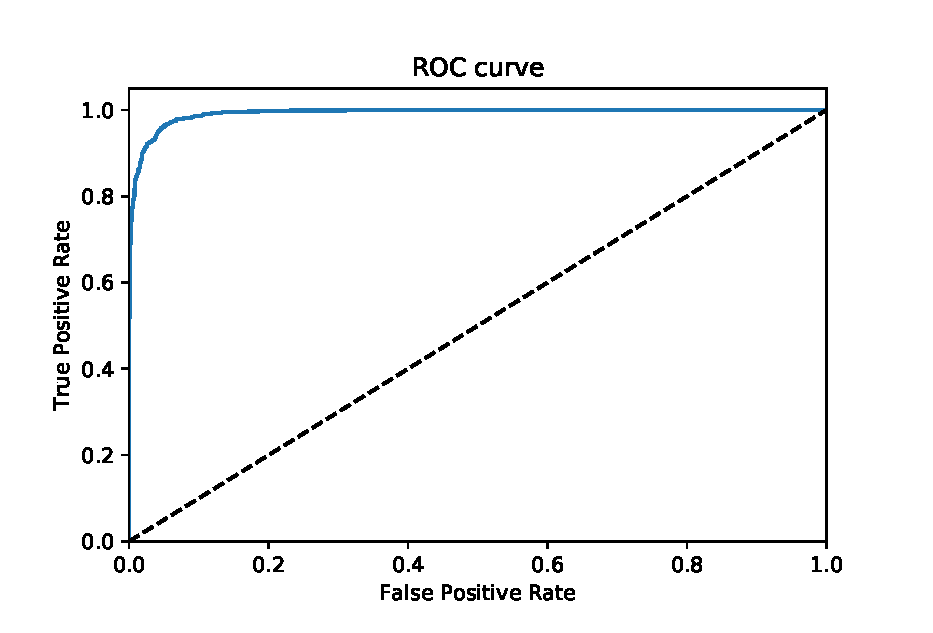
\includegraphics[width=1.0\textwidth]{roc-nmf-soft-svm}
\end{minipage}%
\begin{minipage}{0.5\textwidth}
\includegraphics[width=1.0\textwidth]{conf-mat-nmf-soft-svm}
\end{minipage}
\caption{\emph{Above.} The ROC curve and confusion matrix
of the soft-margin SVM with LSI data.
\emph{Below.} The ROC curve and confusion matrix of the soft-margin SVM
with NMF data.}
\label{fig:soft-svm-2}
\end{figure}

The detailed statistics are shown in the following tables.
\begin{table}[H]
\centering
\begin{tabular}{c|cc}
 & predicted label=0 & predicted label=1 \\ \hline
actual label=0 & 0.00 & 1.00 \\
actual label=1 & 0.00 & 1.00 \\
\end{tabular}
\caption{Confusion matrix for soft-margin SVM with LSI data.}
\end{table}

\begin{table}[H]
\centering
\begin{tabular}{r|cccc}
 & precision & recall & f1-score & support \\ \hline
Computer tech. & 0.00 & 0.00 & 0.00 & 1560 \\
Recreational act. & 0.50 & 1.00 & 0.67 & 1590 \\
avg / total & 0.25 & 0.50 & 0.34 & 3150 \\
\end{tabular}
\caption{Detailed statistics for soft margin SVM with LSI data.}
\end{table}

\begin{table}[H]
\centering
\begin{tabular}{c|cc}
 & predicted label=0 & predicted label=1 \\ \hline
actual label=0 & 0.00 & 1.00 \\
actual label=1 & 0.00 & 1.00 \\
\end{tabular}
\caption{Confusion matrix for soft-margin SVM with NMF data.}
\end{table}

\begin{table}[H]
\centering
\begin{tabular}{r|cccc}
 & precision & recall & f1-score & support \\ \hline
Computer tech. & 0.00 & 0.00 & 0.00 & 1560 \\
Recreational act. & .0.50 & 1.00 & 0.67 & 1590 \\
avg / total & 0.25 & 0.50 & 0.34 & 3150 \\
\end{tabular}
\caption{Detailed statistics for soft margin SVM with NMF data.}
\end{table}

\paragraph{Question (f)}
We report the accuracy result for different penalty terms
in the soft-margin SVMs in the following table.
In our experiment, $k=1000$ is the best choice with both LSI and NMF data.
Figure~\ref{fig:svm-train-2} shows the ROC curves and
confusion matrices with the best choice.
\begin{table}[H]
\centering
\begin{tabular}{cccccccc} \hline
penalty & 0.001 & 0.01 & 0.1 & 1 & 10 & 100 & 1000 \\
accuracy & 0.4577 & 0.4577 & 0.4578 & 0.9344 & 0.9672 & 0.9714 & 0.9598 \\
\hline
\end{tabular}
\end{table}

\begin{figure}[!htb]
\centering
\begin{minipage}{0.5\textwidth}
\includegraphics[width=1.0\textwidth]{roc-lsi-svm-train}
\end{minipage}%
\begin{minipage}{0.5\textwidth}
\includegraphics[width=1.0\textwidth]{conf-mat-lsi-svm-train}
\end{minipage}
\begin{minipage}{0.5\textwidth}
\includegraphics[width=1.0\textwidth]{roc-nmf-svm-train}
\end{minipage}%
\begin{minipage}{0.5\textwidth}
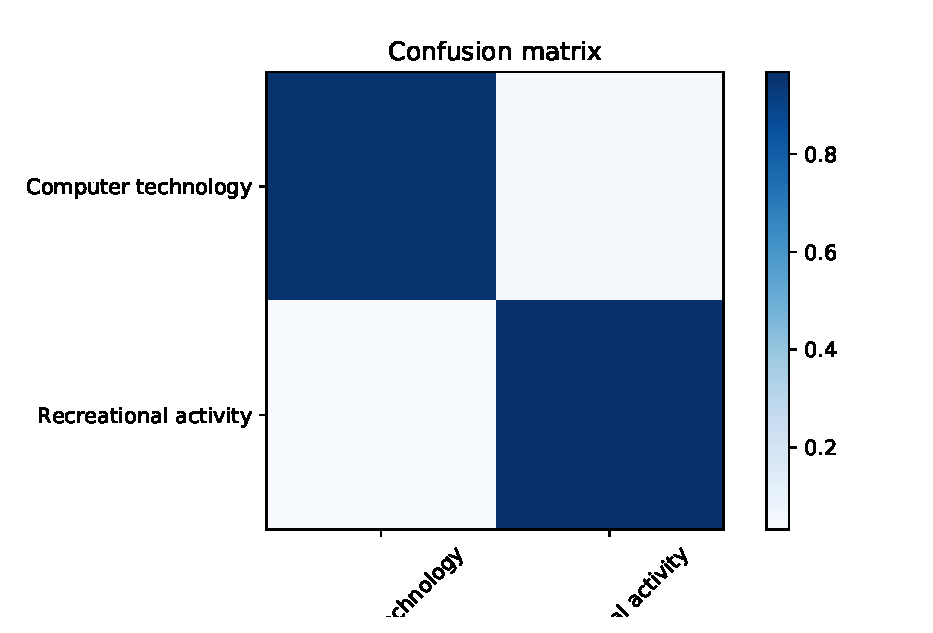
\includegraphics[width=1.0\textwidth]{conf-mat-nmf-svm-train}
\end{minipage}
\caption{\emph{Above.} The ROC curve and confusion matrix
of the best soft-margin SVM with LSI data.
\emph{Below.} The ROC curve and confusion matrix of the best soft-margin SVM
with NMF data.}
\label{fig:svm-train-2}
\end{figure}

The detailed statistics are shown in the following tables.
\begin{table}[H]
\centering
\begin{tabular}{c|cc}
 & predicted label=0 & predicted label=1 \\ \hline
actual label=0 & 0.97 & 0.03 \\
actual label=1 & 0.02 & 0.98 \\
\end{tabular}
\caption{Confusion matrix for best soft-margin SVM with LSI data.}
\end{table}

\begin{table}[H]
\centering
\begin{tabular}{r|cccc}
 & precision & recall & f1-score & support \\ \hline
Computer tech. & 0.98 & 0.97 & 0.97 & 513 \\
Recreational act. & 0.97 & 0.98 & 0.97 & 433 \\
avg / total & 0.97 & 0.97 & 0.97 & 946 \\
\end{tabular}
\caption{Detailed statistics for best soft-margin SVM with LSI data.}
\end{table}

\begin{table}[H]
\centering
\begin{tabular}{c|cc}
 & predicted label=0 & predicted label=1 \\ \hline
actual label=0 & 0.95 & 0.05 \\
actual label=1 & 0.03 & 0.97 \\
\end{tabular}
\caption{Confusion matrix for best soft-margin SVM with NMF data.}
\end{table}

\begin{table}[H]
\centering
\begin{tabular}{r|cccc}
 & precision & recall & f1-score & support \\ \hline
Computer tech. & 0.97 & 0.95 & 0.96 & 513 \\
Recreational act. & 0.95 & 0.97 & 0.96 & 433 \\
avg / total & 0.96 & 0.96 & 0.96 & 946 \\
\end{tabular}
\caption{Detailed statistics for best soft-margin SVM with NMF data.}
\end{table}

\paragraph{Question (g)}
We report the ROC curves and confusion matrices in Figure~\ref{fig:nb-2}.
\begin{figure}[!htb]
\centering
\begin{minipage}{0.5\textwidth}
\includegraphics[width=1.0\textwidth]{roc-lsi-naive-bayes}
\end{minipage}%
\begin{minipage}{0.5\textwidth}
\includegraphics[width=1.0\textwidth]{conf-mat-lsi-naive-bayes}
\end{minipage}
\begin{minipage}{0.5\textwidth}
\includegraphics[width=1.0\textwidth]{roc-nmf-naive-bayes}
\end{minipage}%
\begin{minipage}{0.5\textwidth}
\includegraphics[width=1.0\textwidth]{conf-mat-nmf-naive-bayes}
\end{minipage}
\caption{\emph{Above.} The ROC curve and confusion matrix
of the Gaussian naive Bayes classifier with LSI data.
\emph{Below.} The ROC curve and confusion matrix of the Gaussian naive
Bayes classifier with NMF data.}
\label{fig:nb-2}
\end{figure}

The detailed statistics are shown in the following tables.
\begin{table}[H]
\centering
\begin{tabular}{c|cc}
 & predicted label=0 & predicted label=1 \\ \hline
actual label=0 & 0.87 & 0.13 \\
actual label=1 & 0.05 & 0.95 \\
\end{tabular}
\caption{Confusion matrix for naive Bayes classifier with LSI data.}
\end{table}

\begin{table}[H]
\centering
\begin{tabular}{r|cccc}
 & precision & recall & f1-score & support \\ \hline
Computer tech. & 0.95 & 0.87 & 0.91 & 1560 \\
Recreational act. & 0.88 & 0.95 & 0.92 & 1590 \\
avg / total & 0.92 & 0.91 & 0.91 & 3150 \\
\end{tabular}
\caption{Detailed statistics for naive Bayes classifier with LSI data.}
\end{table}

\begin{table}[H]
\centering
\begin{tabular}{c|cc}
 & predicted label=0 & predicted label=1 \\ \hline
actual label=0 & 0.97 & 0.03 \\
actual label=1 & 0.06 & 0.94 \\
\end{tabular}
\caption{Confusion matrix for naive Bayes classifier with NMF data.}
\end{table}

\begin{table}[H]
\centering
\begin{tabular}{r|cccc}
 & precision & recall & f1-score & support \\ \hline
Computer tech. & 0.94 & 0.97 & 0.95 & 1560 \\
Recreational act. & 0.97 & 0.94 & 0.95 & 1590 \\
avg / total & 0.95 & 0.95 & 0.95 & 3150 \\
\end{tabular}
\caption{Detailed statistics for naive Bayes classifier with NMF data.}
\end{table}

\paragraph{Question (h)}
We report the ROC curves and confusion matrices in Figure~\ref{fig:lr-2}.
\begin{figure}[!htb]
\centering
\begin{minipage}{0.5\textwidth}
\includegraphics[width=1.0\textwidth]{roc-lsi-log-reg}
\end{minipage}%
\begin{minipage}{0.5\textwidth}
\includegraphics[width=1.0\textwidth]{conf-mat-lsi-log-reg}
\end{minipage}
\begin{minipage}{0.5\textwidth}
\includegraphics[width=1.0\textwidth]{roc-nmf-log-reg}
\end{minipage}%
\begin{minipage}{0.5\textwidth}
\includegraphics[width=1.0\textwidth]{conf-mat-nmf-log-reg}
\end{minipage}
\caption{\emph{Above.} The ROC curve and confusion matrix
of the logistic regression classifier with LSI data.
\emph{Below.} The ROC curve and confusion matrix of the logistic regression
classifier with NMF data.}
\label{fig:lr-2}
\end{figure}

The detailed statistics are shown in the following tables.
\begin{table}[H]
\centering
\begin{tabular}{c|cc}
 & predicted label=0 & predicted label=1 \\ \hline
actual label=0 & 0.93 & 0.07 \\
actual label=1 & 0.02 & 0.98 \\
\end{tabular}
\caption{Confusion matrix for logistic regression classifier with LSI data.}
\end{table}

\begin{table}[H]
\centering
\begin{tabular}{r|cccc}
 & precision & recall & f1-score & support \\ \hline
Computer tech. & 0.98 & 0.83 & 0.95 & 1560 \\
Recreational act. & 0.94 & 0.98 & 0.96 & 1590 \\
avg / total & 0.96 & 0.96 & 0.96 & 3150 \\
\end{tabular}
\caption{Detailed statistics for logistic regression classifier
with LSI data.}
\end{table}

\begin{table}[H]
\centering
\begin{tabular}{c|cc}
 & predicted label=0 & predicted label=1 \\ \hline
actual label=0 & 0.93 & 0.07 \\
actual label=1 & 0.02 & 0.98 \\
\end{tabular}
\caption{Confusion matrix for logistic regression classifier with NMF data.}
\end{table}

\begin{table}[H]
\centering
\begin{tabular}{r|cccc}
 & precision & recall & f1-score & support \\ \hline
Computer tech. & 0.98 & 0.93 & 0.95 & 1560 \\
Recreational act. & 0.94 & 0.98 & 0.96 & 1590 \\
avg / total & 0.96 & 0.96 & 0.96 & 3150 \\
\end{tabular}
\caption{Detailed statistics for logistic regression classifier
with NMF data.}
\end{table}

\paragraph{Question (i)}
The following table shows the accuracy results for different penalties
as well as different data.
The result shows that in general the larger penalty coefficient
will generate a better performance,
and overall $\ell_2$ regularization works better than $\ell_1$.

In general, $\ell_2$ regualrization prefers small errors for all examples,
while $\ell_1$ regularization is in favor of sparse solutions
and built-in feature selection.

\paragraph{Question (j)}
We first report the result for multiclass naive Bayes classifier
in Figure~\ref{fig:multi-bayes-2}.
\begin{figure}[!htb]
\centering
\begin{minipage}{0.5\textwidth}
\includegraphics[width=1.0\textwidth]{conf-mat-lsi-multi-bayes}
\end{minipage}%
\begin{minipage}{0.5\textwidth}
\includegraphics[width=1.0\textwidth]{conf-mat-nmf-multi-bayes}
\end{minipage}
\caption{\emph{Left.} The confusion matrix of the multiclass naive
Bayes classifier with LSI data.
\emph{Right.} The confusion matrix of the multiclass naive
Bayes classifier with NMF data.}
\label{fig:multi-bayes-2}
\end{figure}

The detailed statistics are shown in the following tables.
\begin{table}[H]
\centering
\begin{tabular}{cccc}
0.62 & 0.10 & 0.28 & 0.00 \\
0.29 & 0.32 & 0.38 & 0.00 \\
0.12 & 0.12 & 0.76 & 0.00 \\
0.00 & 0.00 & 0.07 & 0.92
\end{tabular}
\caption{Confusion matrix for multiclass naive Bayes classifier
with LSI data.}
\end{table}

\begin{table}[H]
\centering
\begin{tabular}{r|cccc}
& precision & recall & f1-score & support \\ \hline
comp.sys.ibm.pc.hardware & 0.60 & 0.62 & 0.61 & 392 \\
comp.sys.mac.hardware & 0.59 & 0.32 & 0.42 & 385 \\
misc.forsale & 0.51 & 0.76 & 0.96 & 390 \\
soc.rel.christian & 1.00 & 0.92 & 0.96 & 398 \\
avg / total & 0.68 & 0.66 & 0.65 & 1565 \\
\end{tabular}
\caption{Detailed statistics for multiclass naive Bayes classifier
with LSI data.}
\end{table}

\begin{table}[H]
\centering
\begin{tabular}{cccc}
0.86 & 0.04 & 0.10 & 0.00 \\
0.59 & 0.28 & 0.13 & 0.00 \\
0.19 & 0.07 & 0.74 & 0.00 \\
0.07 & 0.01 & 0.02 & 0.89
\end{tabular}
\caption{Confusion matrix for multiclass naive Bayes classifier
with NMF data.}
\end{table}

\begin{table}[H]
\centering
\begin{tabular}{r|cccc}
& precision & recall & f1-score & support \\ \hline
comp.sys.ibm.pc.hardware & 0.50 & 0.86 & 0.63 & 392 \\
comp.sys.mac.hardware & 0.70 & 0.28 & 0.39 & 385 \\
misc.forsale & 0.74 & 0.74 & 0.94 & 390 \\
soc.rel.christian & 1.00 & 0.89 & 0.94 & 398 \\
avg / total & 0.74 & 0.69 & 0.68 & 1565 \\
\end{tabular}
\caption{Detailed statistics for multiclass naive Bayes classifier
with NMF data.}
\end{table}

Figure~\ref{fig:svm-one-2} shows the confusion matrices for SVM
(one-vs-one).
\begin{figure}[!htb]
\centering
\begin{minipage}{0.5\textwidth}
\includegraphics[width=1.0\textwidth]{conf-mat-lsi-svm-one}
\end{minipage}%
\begin{minipage}{0.5\textwidth}
\includegraphics[width=1.0\textwidth]{conf-mat-nmf-svm-one}
\end{minipage}
\caption{\emph{Left.} The confusion matrix of SVM (one-vs-one)
with LSI data.
\emph{Right.} The confusion matrix of SVM (one-vs-one) with NMF data.}
\label{fig:svm-one-2}
\end{figure}

The detailed statistics are shown in the following tables.
\begin{table}[H]
\centering
\begin{tabular}{cccc}
0.84 & 0.10 & 0.06 & 0.00 \\
0.12 & 0.83 & 0.05 & 0.00 \\
0.05 & 0.05 & 0.89 & 0.00 \\
0.01 & 0.01 & 0.01 & 0.98
\end{tabular}
\caption{Confusion matrix for SVM (one-vs-one) with LSI data.}
\end{table}

\begin{table}[H]
\centering
\begin{tabular}{r|cccc}
& precision & recall & f1-score & support \\ \hline
comp.sys.ibm.pc.hardware & 0.82 & 0.84 & 0.83 & 392 \\
comp.sys.mac.hardware & 0.84 & 0.83 & 0.83 & 385 \\
misc.forsale & 0.88 & 0.89 & 0.89 & 390 \\
soc.rel.christian & 0.99 & 0.98 & 0.99 & 398 \\
avg / total & 0.89 & 0.88 & 0.88 & 1565 \\
\end{tabular}
\caption{Detailed statistics for SVM (one-vs-one) with LSI data.}
\end{table}

\begin{table}[H]
\centering
\begin{tabular}{cccc}
0.71 & 0.19 & 0.09 & 0.01 \\
0.15 & 0.77 & 0.06 & 0.01 \\
0.05 & 0.04 & 0.90 & 0.01 \\
0.00 & 0.01 & 0.00 & 0.99
\end{tabular}
\caption{Confusion matrix for SVM (one-vs-one) with NMF data.}
\end{table}

\begin{table}[H]
\centering
\begin{tabular}{r|cccc}
& precision & recall & f1-score & support \\ \hline
comp.sys.ibm.pc.hardware & 0.78 & 0.71 & 0.74 & 392 \\
comp.sys.mac.hardware & 0.76 & 0.77 & 0.77 & 385 \\
misc.forsale & 0.85 & 0.90 & 0.87 & 390 \\
soc.rel.christian & 0.98 & 0.99 & 0.98 & 398 \\
avg / total & 0.84 & 0.84 & 0.84 & 1565 \\
\end{tabular}
\caption{Detailed statistics for SVM (one-vs-one) with NMF data.}
\end{table}

Figure~\ref{fig:svm-rest-2} shows the confusion matrices for SVM
(one-vs-rest).
\begin{figure}[!htb]
\centering
\begin{minipage}{0.5\textwidth}
\includegraphics[width=1.0\textwidth]{conf-mat-lsi-svm-rest}
\end{minipage}%
\begin{minipage}{0.5\textwidth}
\includegraphics[width=1.0\textwidth]{conf-mat-nmf-svm-rest}
\end{minipage}
\caption{\emph{Left.} The confusion matrix of SVM (one-vs-rest)
with LSI data.
\emph{Right.} The confusion matrix of SVM (one-vs-rest) with NMF data.}
\label{fig:svm-rest-2}
\end{figure}

The detailed statistics are shown in the following tables.
\begin{table}[H]
\centering
\begin{tabular}{cccc}
0.82 & 0.11 & 0.06 & 0.01 \\
0.08 & 0.85 & 0.06 & 0.00 \\
0.05 & 0.05 & 0.89 & 0.01 \\
0.01 & 0.01 & 0.01 & 0.98
\end{tabular}
\caption{Confusion matrix for SVM (one-vs-rest) with LSI data.}
\end{table}

\begin{table}[H]
\centering
\begin{tabular}{r|cccc}
& precision & recall & f1-score & support \\ \hline
comp.sys.ibm.pc.hardware & 0.85 & 0.82 & 0.84 & 392 \\
comp.sys.mac.hardware & 0.84 & 0.85 & 0.85 & 385 \\
misc.forsale & 0.87 & 0.89 & 0.88 & 390 \\
soc.rel.christian & 0.98 & 0.98 & 0.98 & 398 \\
avg / total & 0.89 & 0.89 & 0.89 & 1565 \\
\end{tabular}
\caption{Detailed statistics for SVM (one-vs-rest) with LSI data.}
\end{table}

\begin{table}[H]
\centering
\begin{tabular}{cccc}
0.52 & 0.29 & 0.12 & 0.06 \\
0.04 & 0.83 & 0.07 & 0.05 \\
0.03 & 0.05 & 0.90 & 0.02 \\
0.00 & 0.01 & 0.00 & 0.99
\end{tabular}
\caption{Confusion matrix for SVM (one-vs-rest) with NMF data.}
\end{table}

\begin{table}[H]
\centering
\begin{tabular}{r|cccc}
& precision & recall & f1-score & support \\ \hline
comp.sys.ibm.pc.hardware & 0.88 & 0.52 & 0.66 & 392 \\
comp.sys.mac.hardware & 0.70 & 0.83 & 0.76 & 385 \\
misc.forsale & 0.82 & 0.90 & 0.86 & 390 \\
soc.rel.christian & 0.88 & 0.99 & 0.94 & 398 \\
avg / total & 0.82 & 0.81 & 0.80 & 1565 \\
\end{tabular}
\caption{Detailed statistics for SVM (one-vs-rest) with NMF data.}
\end{table}

\end{document}
